
\chapter{Electrical activity in the brain}

In this chapter we will discuss how brain activity can be measured and where the measurable activity originates from. We will also compare different neuroimaging techniques and choose the neuroimaging device most suitable for our needs. 

\section{Source of the electrical activity}
\label{sec:neuron}

As all living organisms are composed of cells, so are humans and the human brain. The brain consists of nerve cells called neurons and non-neural cells. There are approximately 86 billion neurons in the human brain and roughly as much non-neural cells \cite{neuroncount}. A typical neuron has a cell body, multiple nerve endings or dendrites, and one nerve fibre or axon. Both dendrites and axons can branch multiple times. 

\begin{figure}[b!]
	\centering
	\begin{subfigure}{0.48\textwidth}
		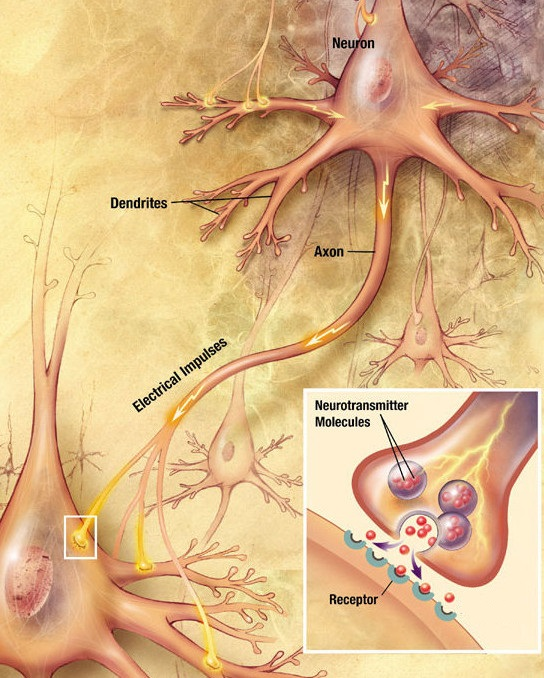
\includegraphics[width=\textwidth]{synapse_modified.jpg}
		\caption{Neurons and a chemical synapse \cite[p.~17]{neuronpic}}
		\label{fig:neuron_synapse}
	\end{subfigure}
	~
	\begin{subfigure}{0.48\textwidth}
		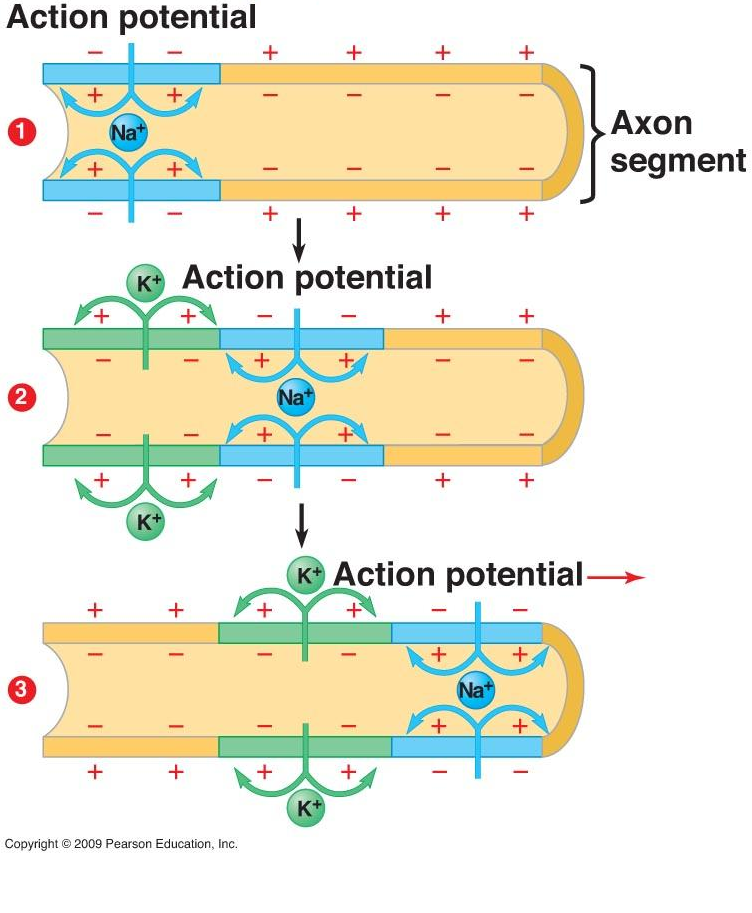
\includegraphics[width=\textwidth]{action_potential.png}
		\caption{Action potential \cite{action_potential_pic}}
		\label{fig:action_potential}
	\end{subfigure}
	\caption{The structure of a neuron}
\end{figure}

Neurons interact with each other via electro-chemical signals that are transmitted through various connections. These connections are not static and can change over time. Functionally related neurons are connected to each other and form neural pathways \cite{neuralpathway}. The general rule is that a neuron sends signals through its axon and receives signals through dendrites. The connection between an axon and a dendrite is called a synapse. See figure \ref{fig:neuron_synapse} for an example of neurons and a synapse.

To send signals, neurons must be able to maintain electrical potential called membrane potential. Membrane potential is the difference in electric potential between the interior and the exterior of a cell. When neurons are not sending signals, their membrane potentials are slightly negative. The membrane potential of a neuron at a resting state is called resting potential. Negative resting potential is achieved by having more positively charged ions around the cell than inside the cell.

By having stable resting potential, a neuron is able to send signals by rapidly increasing and decreasing the membrane potential along an axon. Therefore, the signal travelling along an axon is actually higher membrane potential. This event is called an action potential. See figure \ref{fig:action_potential} for illustration. To increase or decrease the membrane potential of a cell, ionophoric proteins are used. These proteins transport ions across the cell membrane to regulate the concentration of ions and membrane potential.

Action potential is initiated by a certain threshold voltage called threshold potential. When the membrane potential of a neuron exceeds threshold potential, the neuron sends signals to other cells. The neuron that receives the signal is called postsynaptic cell. Synaptic input in a postsynaptic cell can cause the membrane potential of the postsynaptic cell to increase or decrease. This change in membrane potential is called a postsynaptic potential and it can cause an action potential in the postsynaptic cell.

The following paragraph is mainly based on article \cite{electric_field}. Postsynaptic potentials cause small current flows into the cell. To achieve electroneutrality, a balancing current from the interior to the exterior of the cell is needed. Ions enter the cell from a location called sink and flow to the exterior of the cell to a location called source. A sink and a source form a dipole. See figure \ref{fig:dipole_electric} for illustration. These dipoles are important because it is possible to measure the electric field produced by these dipoles from the scalp. See figure \ref{fig:dipole_neuron} for illustration. Measuring these electric fields is further discussed in section \ref{sec:EEG}. Although action potentials generate stronger currents than postsynaptic potentials, their duration is low and nearby neurons rarely fire synchronously.

\begin{figure}[h!]
	\centering
	\begin{subfigure}{0.48\textwidth}
		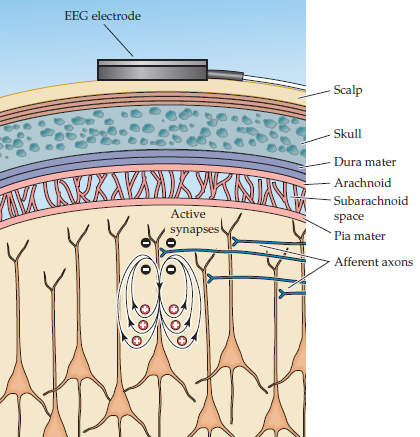
\includegraphics[width=\textwidth]{dipole_neuron.png}
		\caption{Dipole generated by a neuron \cite[p.~669]{neuroscience}}
		\label{fig:dipole_neuron}
	\end{subfigure}
	~
	\begin{subfigure}{0.48\textwidth}
		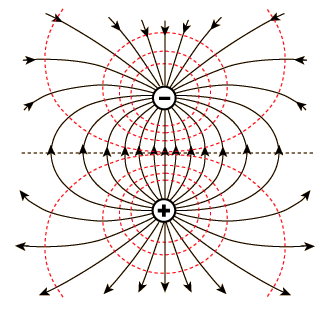
\includegraphics[width=\textwidth]{dipole_electric.png}
		\caption{The electric field of a dipole\protect\footnotemark}
		\label{fig:dipole_electric}
	\end{subfigure}
	\caption{Dipoles}
	\label{fig:dipole}
\end{figure}
\footnotetext{http://hyperphysics.phy-astr.gsu.edu/hbase/electric/equipot.html}

\section{Functional neuroimaging}
\label{sec:neuroimaging}

As discussed in section \ref{sec:neuron}, neurons in the brain are sending electrochemical signals to communicate with each other. There are several techniques available to measure this activity. We will give a brief overview of various methods before continuing to discuss the biological background. Measuring an aspect of brain function is called functional neuroimaging and common measurement methods divide into haemodynamic and electromagnetic techniques.

Haemodynamic techniques measure blood oxygenation and blood flow in the brain. More oxygen has to be delivered to more active brain regions and this allows the brain activity to be measured. Haemodynamic techniques include \gls{fMRI}, \gls{fNIRS}, \gls{PET}.

Electromagnetic techniques measure either electrical activity or magnetic fields produced by the electrical activity along the scalp. Electromagnetic techniques include \gls{EEG} and \gls{MEG}. These methods have lower temporal resolution than haemodynamic methods, but measure only the activity in the outer layer of the brain. Temporal resolution is the smallest time period of neural activity that is reliably separated out by measuring technique.
%http://psychcentral.com/lib/types-of-brain-imaging-techniques/0001057
%http://www.macalester.edu/academics/psychology/whathap/UBNRP/Imaging/eeg.html
%http://scienceforthemasses.org/2014/04/11/selecting-an-eeg-device/

To decide which method is best for controlling a robot, we will compare cost, portability and temporal resolution of each method. See table \ref{tab:neuroimaging} for details. For real-time robot controlling, lower temporal resolution is better because it enables faster decision making. We also prefer techniques that are portable and available for the consumer, so the usage would not be limited to certain location and would be available to the people in need. Considering all these arguments, it can be seen that the best choice for controlling a robot is an \gls{EEG} device.

% Constants for table

\newcommand{\pMEG}{\tablefootnote{http://neurogadget.com/2012/12/15/inexpensive-magnetoencephalography-meg-system-could-be-available-at-every-hospital/6495}}
\newcommand{\pfMRI}{\tablefootnote{http://info.blockimaging.com/bid/92623/MRI-Machine-Cost-and-Price-Guide}}
\newcommand{\pPET}{\tablefootnote{http://info.blockimaging.com/bid/68875/How-Much-Does-a-PET-CT-Scanner-Cost}}
\newcommand{\pEEG}{\tablefootnote{http://en.wikipedia.org/wiki/Comparison\_of\_consumer\_brain-computer\_interfaces}}
\newcommand{\pNIRS}{\cite{NIRS}}
\newcommand{\tresol}{\cite{timeresol}}

% Table

\begin{table}[h]
	\centering
	\begin{tabular}{|c|c|c|c|c|c|}\hline
			& Price	from				& Portable	& Temporal resolution		& Special requirements			\\\hline
\gls{MEG}	& millions\pMEG				& no		& milliseconds \tresol		& magnetically shielded room	\\\hline
\gls{fMRI}	& \SI{150000}[\$]\pfMRI		& no		& about 1 second \tresol	& magnetically shielded room	\\\hline
\gls{PET}	& \SI{125000}[\$]\pPET		& no		& about 1 second \tresol	& radioactive isotopes injection\\\hline
\gls{fNIRS}	& \SI{10000}[\$]{} \pNIRS	& yes		& over 0.1 second \pNIRS	&								\\\hline
\gls{EEG}	& \SI{45}[\$]\pEEG			& yes		& milliseconds \tresol		&								\\\hline
	\end{tabular}
	\caption{Comparison of functional neuroimaging methods}
	\label{tab:neuroimaging}
\end{table}

\section{Electroencephalography}
\label{sec:EEG}

As already mentioned in the previous section, \gls{EEG} measures the electrical activity along the scalp. This electrical activity originates mainly from the electric fields generated by neurons as discussed in section \ref{sec:neuron}. However, the electric potential generated by one neuron is far too low to be recognized. Therefore, approximately 108 neurons have to have synchronous electrical activity to a create measurable field \cite{field_count}. Furthermore, these neurons have to have certain orientation for the electric fields to add up and reach the electrode on the scalp. See figure \ref{fig:dipole_neuron} for example.

\gls{EEG} measures the potential fields as the function of voltage versus time using electrodes placed on scalp \cite{field_count}. Since voltage is the electrical potential difference between two points, one or more reference electrodes should be used. Then voltmeter can be used to measure the differences in voltage between two electrodes, one of which is the reference electrode. See figure \ref{fig:voltmeter} for a simplified scheme.

Usually electrodes are placed on the scalp according to international 10-20 electrode location system. The outer layer of the brain can be classified into four lobes: temporal, occipital, parietal and frontal. See figure \ref{fig:brain_lobes} for example. 10-20 electrode location system uses a letter and a number to identify electrode location. The letter is the first letter of the brain lobe above which the electrode is located and therefore the electrode measures the activity of this brain lobe. There are more complicated electrode-naming-systems that extend the 10-20 system. See figure \ref{fig:electrode_locations} for illustration.

In a broad sense, \gls{EEG} recording is linked to the state of the general activation of the brain \cite{VEP}. Therefore, due to the generality of the recording, we cannot see potentials evoked by certain events in the recording because the general fluctuations are much larger than the evoked potential. A brain potential evoked by some event is called \gls{ERP}. \glspl{ERP} are associated with the information flow in the cortical areas and are usually obtained by an averaging technique \cite{ERP}. \glspl{ERP} are time locked to a stimulus event and therefore may be recorded by presenting a stimulus with a certain time interval to a subject and calculating the average of \gls{EEG} signals recorded in the same time interval.

\begin{figure}[h]
	\centering
	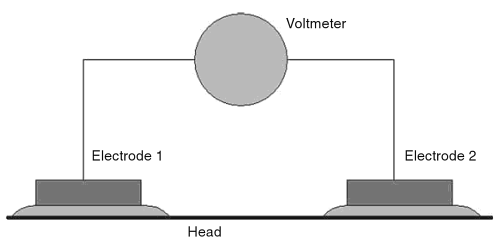
\includegraphics[width=0.70\textwidth]{voltmeter.png}
	\caption{Electrodes connected to a voltmeter \cite[p.~120]{ERP}}
	\label{fig:voltmeter}
\end{figure}

\section{Visual evoked potential}

In section \ref{sec:EEG} we gave a brief overview of \glspl{ERP}. Now we are going to discuss one specific \gls{ERP} called \gls{VEP}. As the name suggests, \glspl{VEP} are elicited by visual stimuli. The visual stimulus for eliciting a \gls{VEP} can be very simple, for example a white square blinking on a black computer screen.

The visual processing centre is located in the back of the brain. The corresponding brain lobe is called occipital lobe. Therefore, when subject sees the stimulus, the signal travels from the eyes to the visual processing centre through the primary visual pathway \cite{neuroscience}. See figure \ref{fig:lobes_pathway} for illustration. The primary visual pathway is a neural pathway; neural pathways were also mentioned in the section \ref{sec:neuron}.

Due to the posterior location of the occipital lobe, electrodes must be placed to the back of the head when recording \glspl{VEP} with \gls{EEG}. These electrode locations are identified with the letter O as discussed in section \ref{sec:EEG}.

When comparing the \glspl{VEP} elicited in the central visual field and in the peripheral vision by the same stimuli, it can be seen that the stimulation of the central visual field produces larger \glspl{VEP} \cite{VEP_size}. This allows us to present multiple visual stimuli to a subject and detect which stimulus is the subject looking at. 

To make the detection of \glspl{VEP} easier, \glspl{SSVEP} are used. If the visual stimulus is presented at a constant rate and the rate is so fast that the visual pathway cannot recover before the next stimulus is presented, then the elicited response becomes continuous and it is called the \gls{SSVEP} \cite{VEP}. See figure X for an example of \gls{VEP} and \gls{SSVEP}. \glspl{SSVEP} are sinusoidal and therefore it is easier to detect it than \glspl{VEP}, which have more complex shape and are not continuous.

\begin{figure}[h]
	\centering
	\begin{subfigure}{0.48\textwidth}
		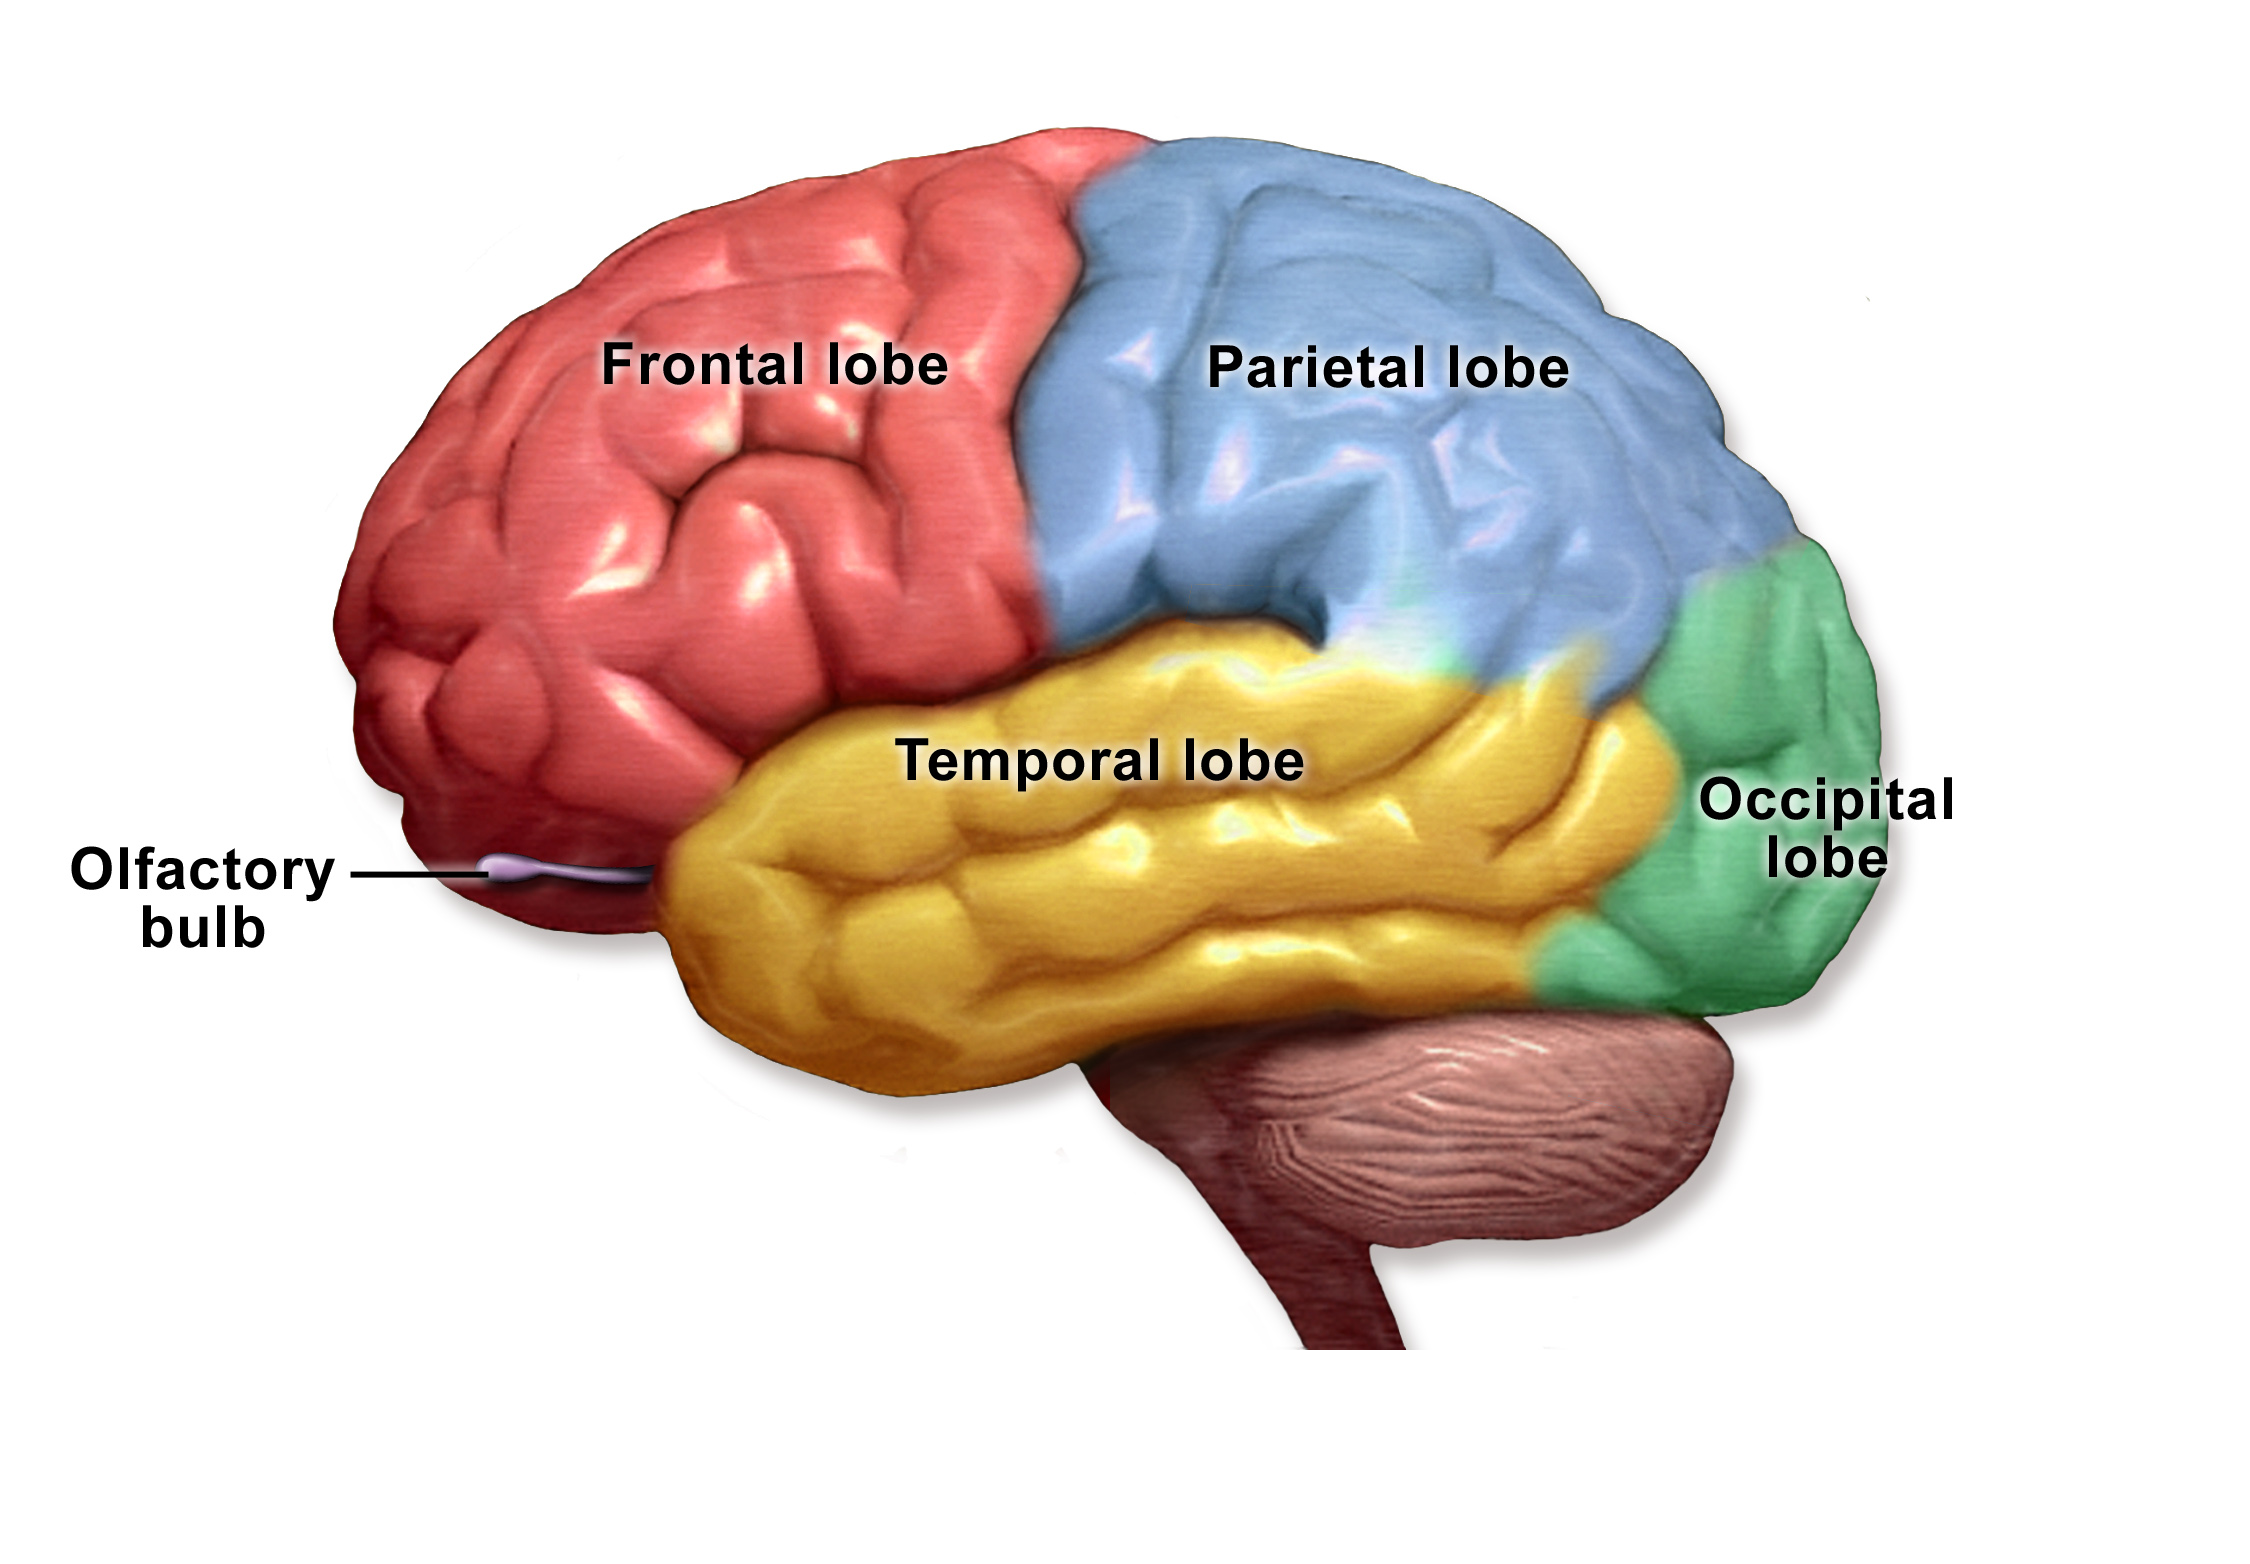
\includegraphics[width=\textwidth]{brain_lobes.png}
		\caption{Lobes of the brain \cite{blausen}}
		\label{fig:brain_lobes}
	\end{subfigure}
	~
	\begin{subfigure}{0.48\textwidth}
		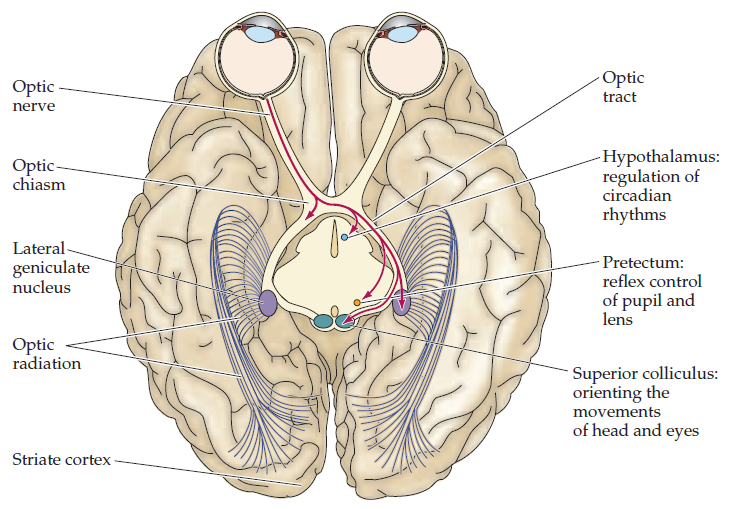
\includegraphics[width=\textwidth]{visual_pathway.png}
		\caption{The primary visual pathway \cite[p.~261]{neuroscience}}
		\label{fig:visual_pathway}
	\end{subfigure}
	\caption{The location of occipital lobe and the neural pathway from eyes to the lobe}
	\label{fig:lobes_pathway}
\end{figure}

\section{Emotiv EPOC}

In section \ref{sec:neuroimaging} we briefly compared different functional neuroimaging methods and concluded that currently \gls{EEG} is most suitable for our needs. But there is a wide variety of EEG devices available. See table \ref{tab:EEG} for details. As discussed in section \ref{sec:neuroimaging}, we prefer a device that is available to the consumer.

OpenBCI is an open source brain-computer interface that provides access to all the data and algorithms, which makes it good for specialists, but it is not easy to use for a non-specialist. From the more consumer-friendly devices, Emotiv EPOC seems to offer good price-quality relationship.

Emotiv EPOC has 16 electrodes, two of which are reference electrodes. Reference electrodes have two different possible locations: P3 and P4 or locations behind the ears. Other electrodes have fixed locations AF3, AF4, F3, F4, F7, F8, FC5, FC6, P7, P8, T7, T8, O1, O2. See figure \ref{fig:electrode_locations} for illustration. Emotiv EPOC has a sampling rate of \SI{128}{Hz}, an internal sampling rate of \SI{2048}{Hz} and an \gls{ADC} resolution of 16 bit. 

An \gls{ADC} device converts continuous voltage to the sequence of discrete values or in other words, an analog signal to a digital signal that can be processed by a computer. The \gls{ADC} resolution indicates the number of discrete values it can produce. Sampling rate is the rate at which digital values are extracted from a continuous signal.

\newcommand{\patiCHamp}{\tablefootnote{http://www.brainvision.com/files/actiCHamp-PyCorder-Flyer\_US.pdf}}
\newcommand{\pmitsar}{\tablefootnote{http://www.novatecheeg.com/products--software.html}}
\newcommand{\pemotiv}{\tablefootnote{https://emotiv.com/epoc.php}}
\newcommand{\pmindwave}{\tablefootnote{http://store.neurosky.com/products/mindwave-1}}
\newcommand{\mitsarspec}{\tablefootnote{http://www.mitsar-medical.com/eeg-machine/eeg-amplifier-compare/}}
\newcommand{\popenbci}{\tablefootnote{http://openbci.myshopify.com/products/openbci-8-bit-board-kit}}

\begin{table}[h]
	\centering
	\begin{tabular}{|c|c|c|c|c|}\hline
								& Price						& Channels	& Sampling rate	& \gls{ADC} resolution	\\\hline
		Mindwave\pmindwave		& \SI{80}[\$]				& 1			& \SI{512}{Hz}	& 12 bit				\\\hline
		Emotiv EPOC\pemotiv		& \SI{400}[\$]				& 14+2		& \SI{128}{Hz}	& 16 bit				\\\hline
		OpenBCI\popenbci		& \SI{450}[\$]				& 8			& adjustable	& 24 bit				\\\hline
		Mitsar 202\mitsarspec	& \SI{10500}[\$]\pmitsar	& 31+1		& \SI{2}{kHz}	& 24 bit				\\\hline
		atiCHamp\patiCHamp		& \SI{77100}[\$]			& 160		& \SI{25}{kHZ}	& 24 bit				\\\hline
	\end{tabular}
	\caption{Comparison of EEG devices}
	\label{tab:EEG}
\end{table}

\begin{figure}[h]
	\centering
	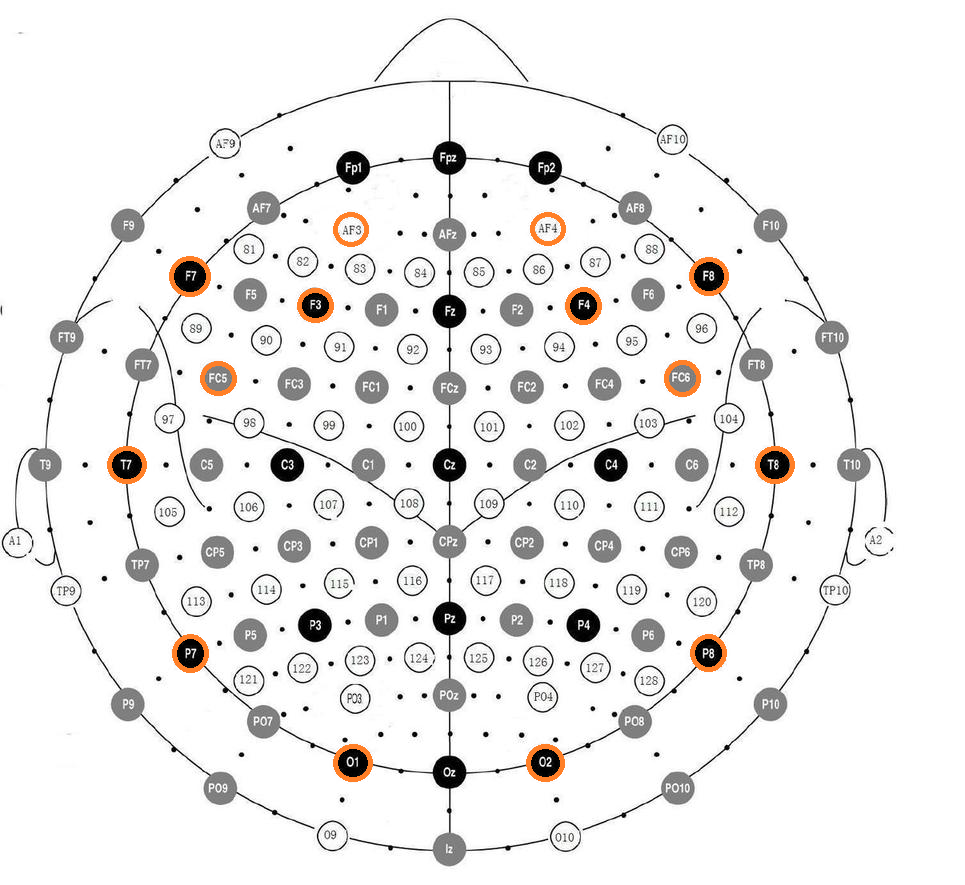
\includegraphics[width=0.7\textwidth]{electrode_locations.png}
	\caption{Electrode locations used by Emotiv EPOC\protect\footnotemark}
	\label{fig:electrode_locations}
\end{figure}
\footnotetext{http://emotiv.wikia.com/wiki/Emotiv\_EPOC}
